% Options for packages loaded elsewhere
\PassOptionsToPackage{unicode}{hyperref}
\PassOptionsToPackage{hyphens}{url}
%
\documentclass[
]{book}
\usepackage{amsmath,amssymb}
\usepackage{iftex}
\ifPDFTeX
  \usepackage[T1]{fontenc}
  \usepackage[utf8]{inputenc}
  \usepackage{textcomp} % provide euro and other symbols
\else % if luatex or xetex
  \usepackage{unicode-math} % this also loads fontspec
  \defaultfontfeatures{Scale=MatchLowercase}
  \defaultfontfeatures[\rmfamily]{Ligatures=TeX,Scale=1}
\fi
\usepackage{lmodern}
\ifPDFTeX\else
  % xetex/luatex font selection
\fi
% Use upquote if available, for straight quotes in verbatim environments
\IfFileExists{upquote.sty}{\usepackage{upquote}}{}
\IfFileExists{microtype.sty}{% use microtype if available
  \usepackage[]{microtype}
  \UseMicrotypeSet[protrusion]{basicmath} % disable protrusion for tt fonts
}{}
\makeatletter
\@ifundefined{KOMAClassName}{% if non-KOMA class
  \IfFileExists{parskip.sty}{%
    \usepackage{parskip}
  }{% else
    \setlength{\parindent}{0pt}
    \setlength{\parskip}{6pt plus 2pt minus 1pt}}
}{% if KOMA class
  \KOMAoptions{parskip=half}}
\makeatother
\usepackage{xcolor}
\usepackage{longtable,booktabs,array}
\usepackage{calc} % for calculating minipage widths
% Correct order of tables after \paragraph or \subparagraph
\usepackage{etoolbox}
\makeatletter
\patchcmd\longtable{\par}{\if@noskipsec\mbox{}\fi\par}{}{}
\makeatother
% Allow footnotes in longtable head/foot
\IfFileExists{footnotehyper.sty}{\usepackage{footnotehyper}}{\usepackage{footnote}}
\makesavenoteenv{longtable}
\usepackage{graphicx}
\makeatletter
\def\maxwidth{\ifdim\Gin@nat@width>\linewidth\linewidth\else\Gin@nat@width\fi}
\def\maxheight{\ifdim\Gin@nat@height>\textheight\textheight\else\Gin@nat@height\fi}
\makeatother
% Scale images if necessary, so that they will not overflow the page
% margins by default, and it is still possible to overwrite the defaults
% using explicit options in \includegraphics[width, height, ...]{}
\setkeys{Gin}{width=\maxwidth,height=\maxheight,keepaspectratio}
% Set default figure placement to htbp
\makeatletter
\def\fps@figure{htbp}
\makeatother
\setlength{\emergencystretch}{3em} % prevent overfull lines
\providecommand{\tightlist}{%
  \setlength{\itemsep}{0pt}\setlength{\parskip}{0pt}}
\setcounter{secnumdepth}{5}
\usepackage{booktabs}
\ifLuaTeX
  \usepackage{selnolig}  % disable illegal ligatures
\fi
\usepackage[]{natbib}
\bibliographystyle{plainnat}
\IfFileExists{bookmark.sty}{\usepackage{bookmark}}{\usepackage{hyperref}}
\IfFileExists{xurl.sty}{\usepackage{xurl}}{} % add URL line breaks if available
\urlstyle{same}
\hypersetup{
  pdftitle={AI Declassified: A Ross Faculty Survival Guide},
  pdfauthor={Adam Zhang, Ryan Berger, Michelle Xu, Fuad Chedid, Sona Coshal},
  hidelinks,
  pdfcreator={LaTeX via pandoc}}

\title{AI Declassified: A Ross Faculty Survival Guide}
\author{Adam Zhang, Ryan Berger, Michelle Xu, Fuad Chedid, Sona Coshal}
\date{2023-07-29}

\begin{document}
\maketitle

{
\setcounter{tocdepth}{1}
\tableofcontents
}
\hypertarget{introduction}{%
\chapter{Introduction}\label{introduction}}

This book is intended to be a comprehensive look at the challenges faced by Ross faculty regarding the advent of Generative AI in academia. The content of this book is based on real world problems, solutions, and ideas captured from research and interviews with Ross Faculty members who are currently contending with the challenges brought on by educating in the age of Generative AI.

\hypertarget{about-us}{%
\chapter{About Us}\label{about-us}}

\hypertarget{ryan-berger}{%
\section{Ryan Berger}\label{ryan-berger}}

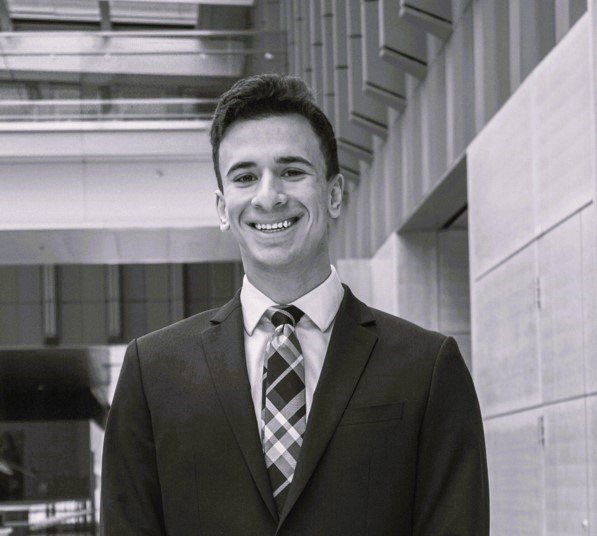
\includegraphics[width=0.4\linewidth]{rtberger}

Hey! I'm Ryan Berger. I am a current Master's of Business Analytics student at Michigan Ross, and also attended Michigan for my undergrad in the School of Information. I am from New Jersey, which means I am a Giants fan and I like to say I'm from New York.

\hypertarget{adam-zhang}{%
\section{Adam Zhang}\label{adam-zhang}}

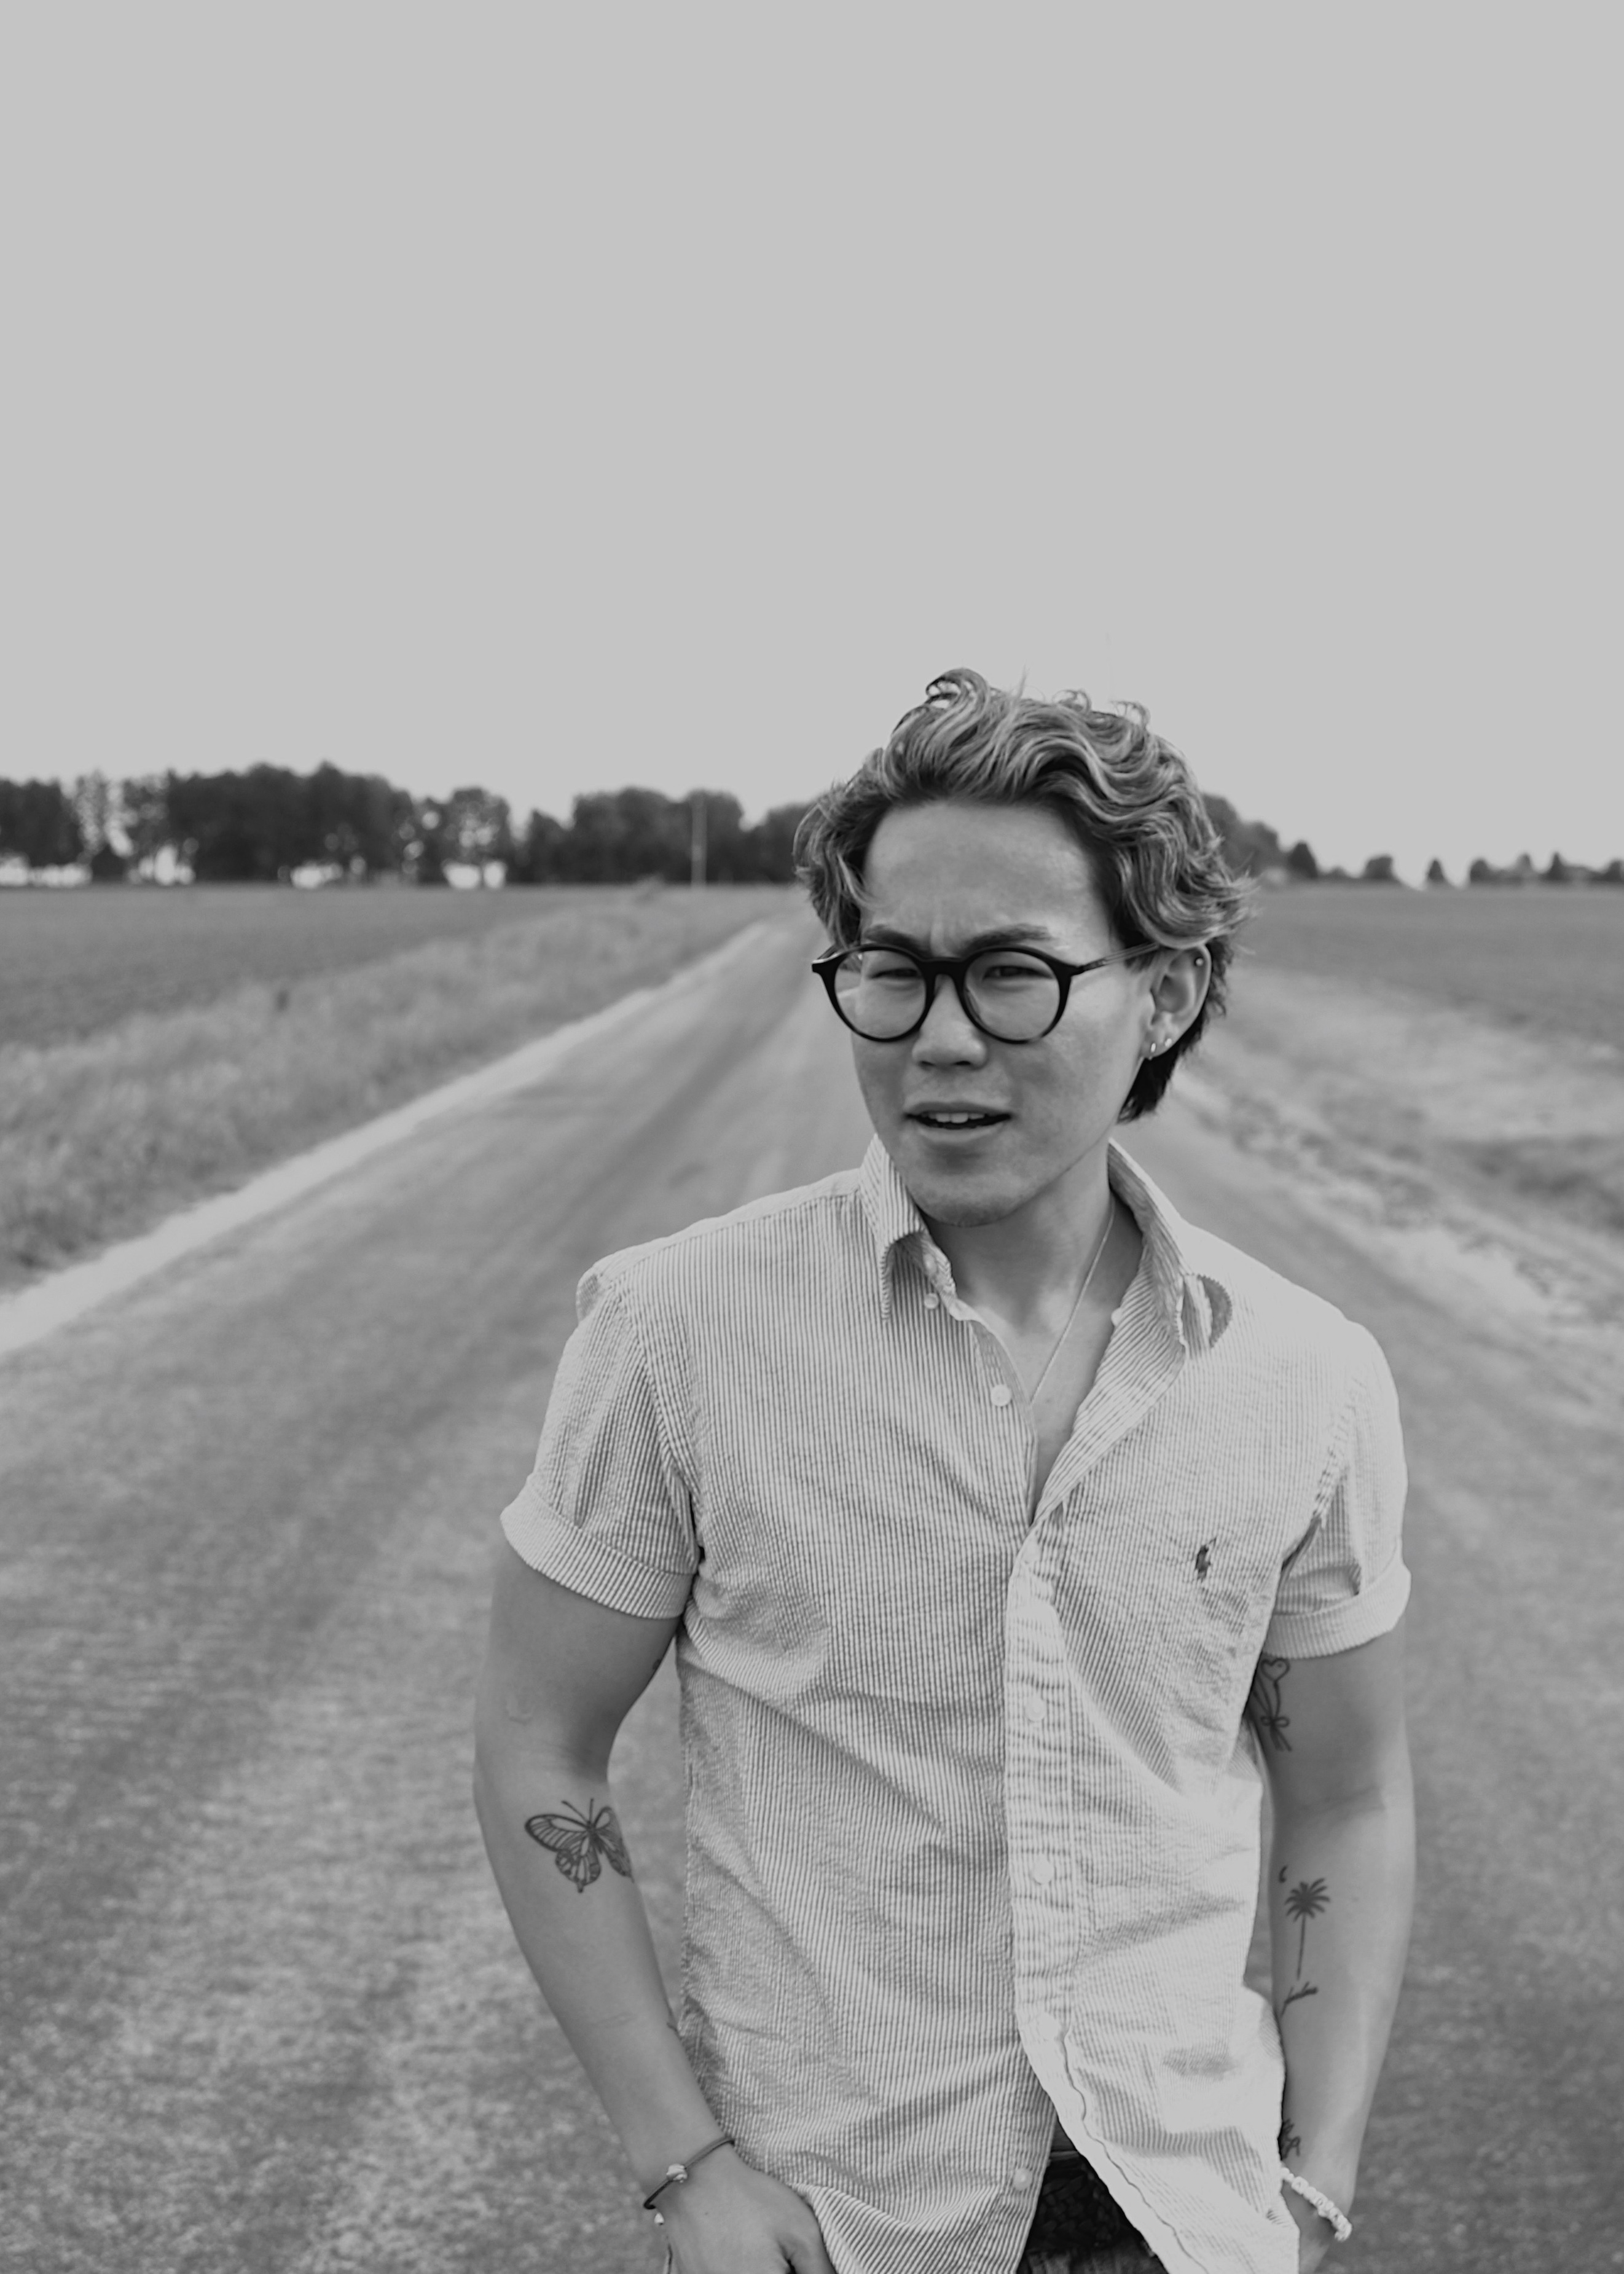
\includegraphics[width=0.4\linewidth]{AZ}

Hi! I'm Adam

\hypertarget{michelle-xu}{%
\section{Michelle Xu}\label{michelle-xu}}

Hello, I'm Michelle Xu, originally from China. I spent six years living in the beautiful city of San Diego, California. After high school, I moved to Ann Arbor, Michigan, to pursue a major in Bioinformatics at LS\&A. Currently, I'm a Master of Business Analytics student at the University of Michigan, Ross School of Business.

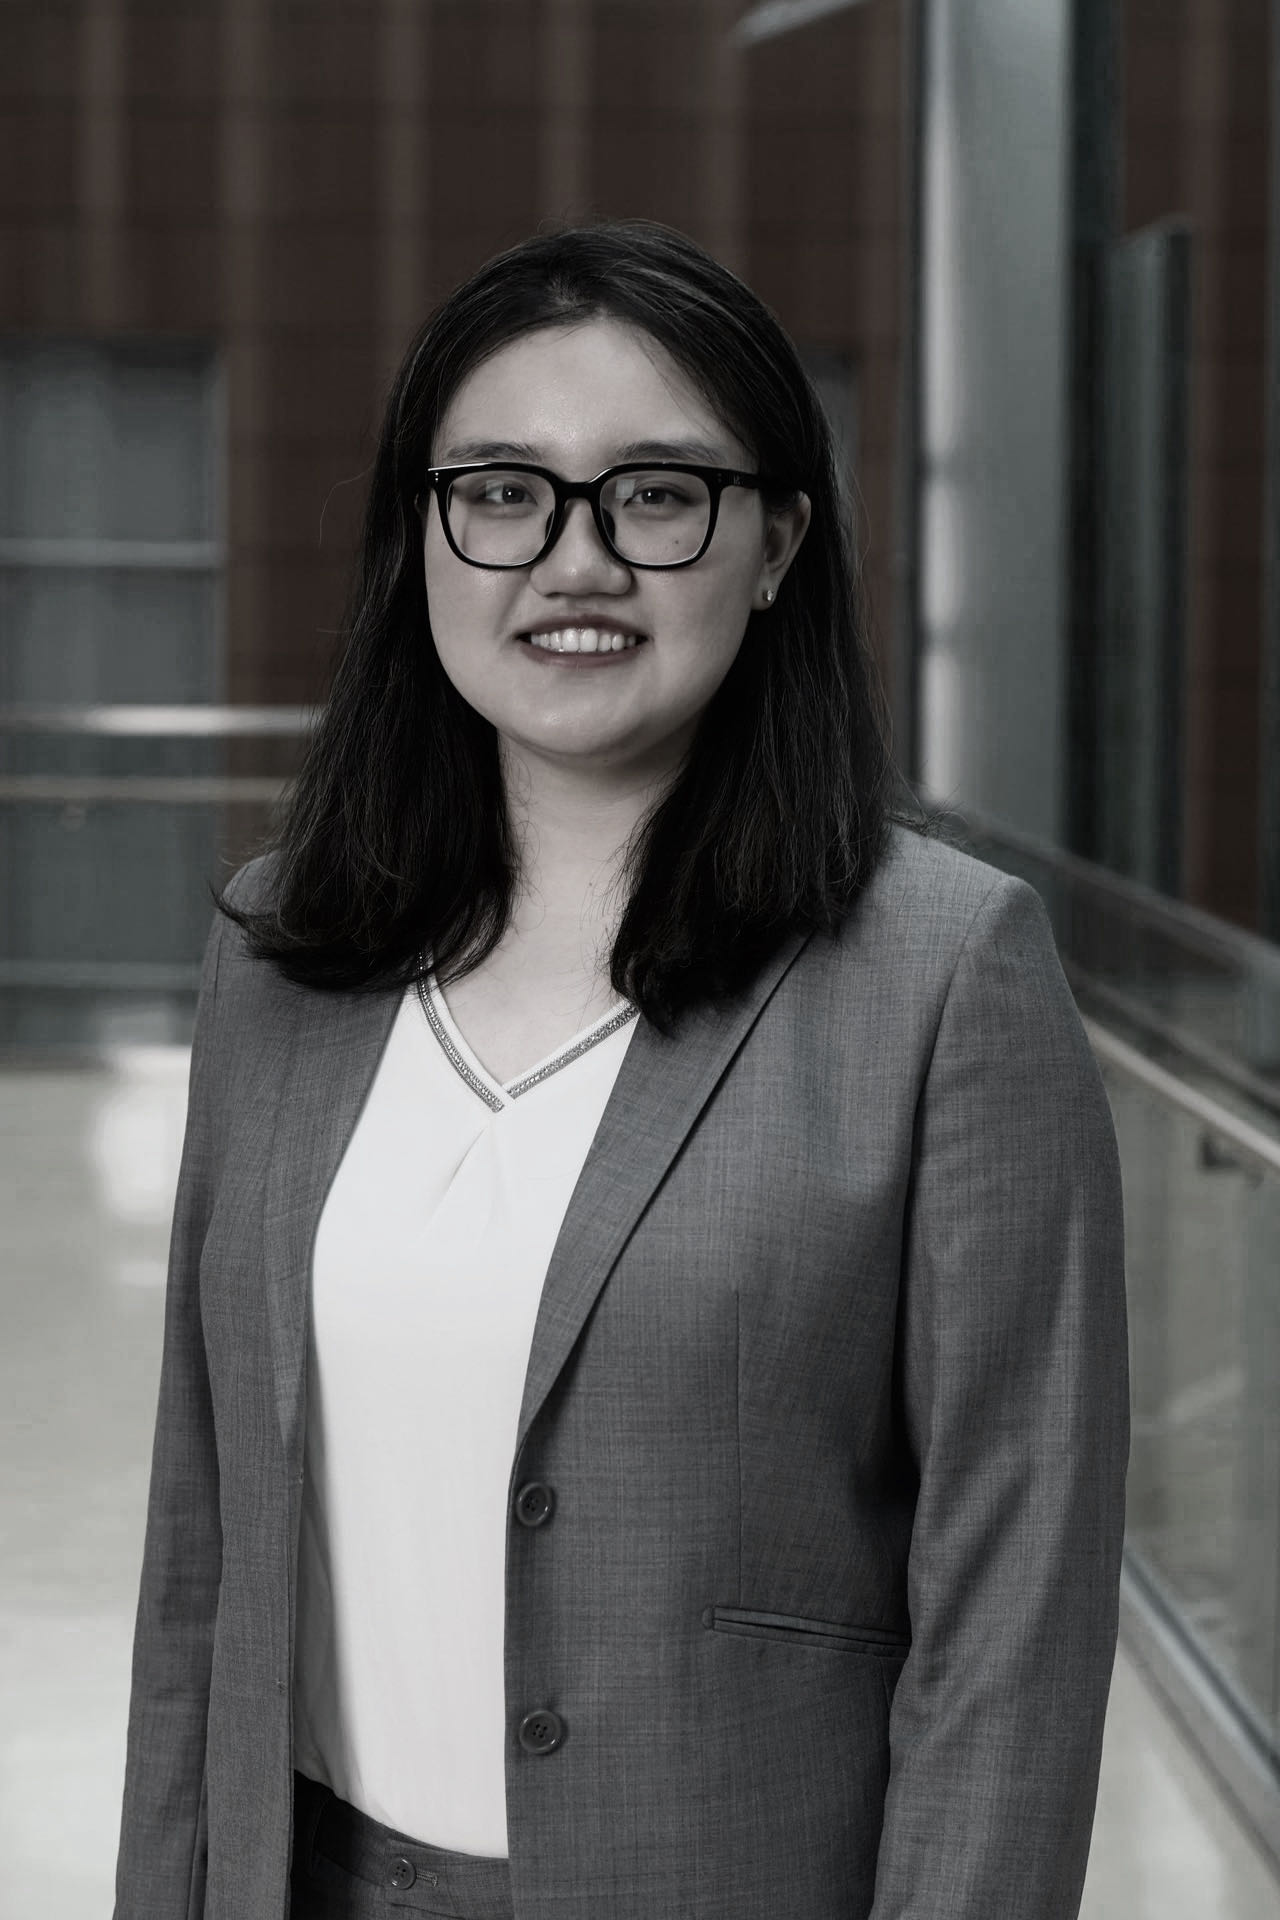
\includegraphics[width=0.4\linewidth]{WechatIMG10}

\hypertarget{sona-coshal}{%
\section{Sona Coshal}\label{sona-coshal}}

\hypertarget{fuad-chedid}{%
\section{Fuad Chedid}\label{fuad-chedid}}

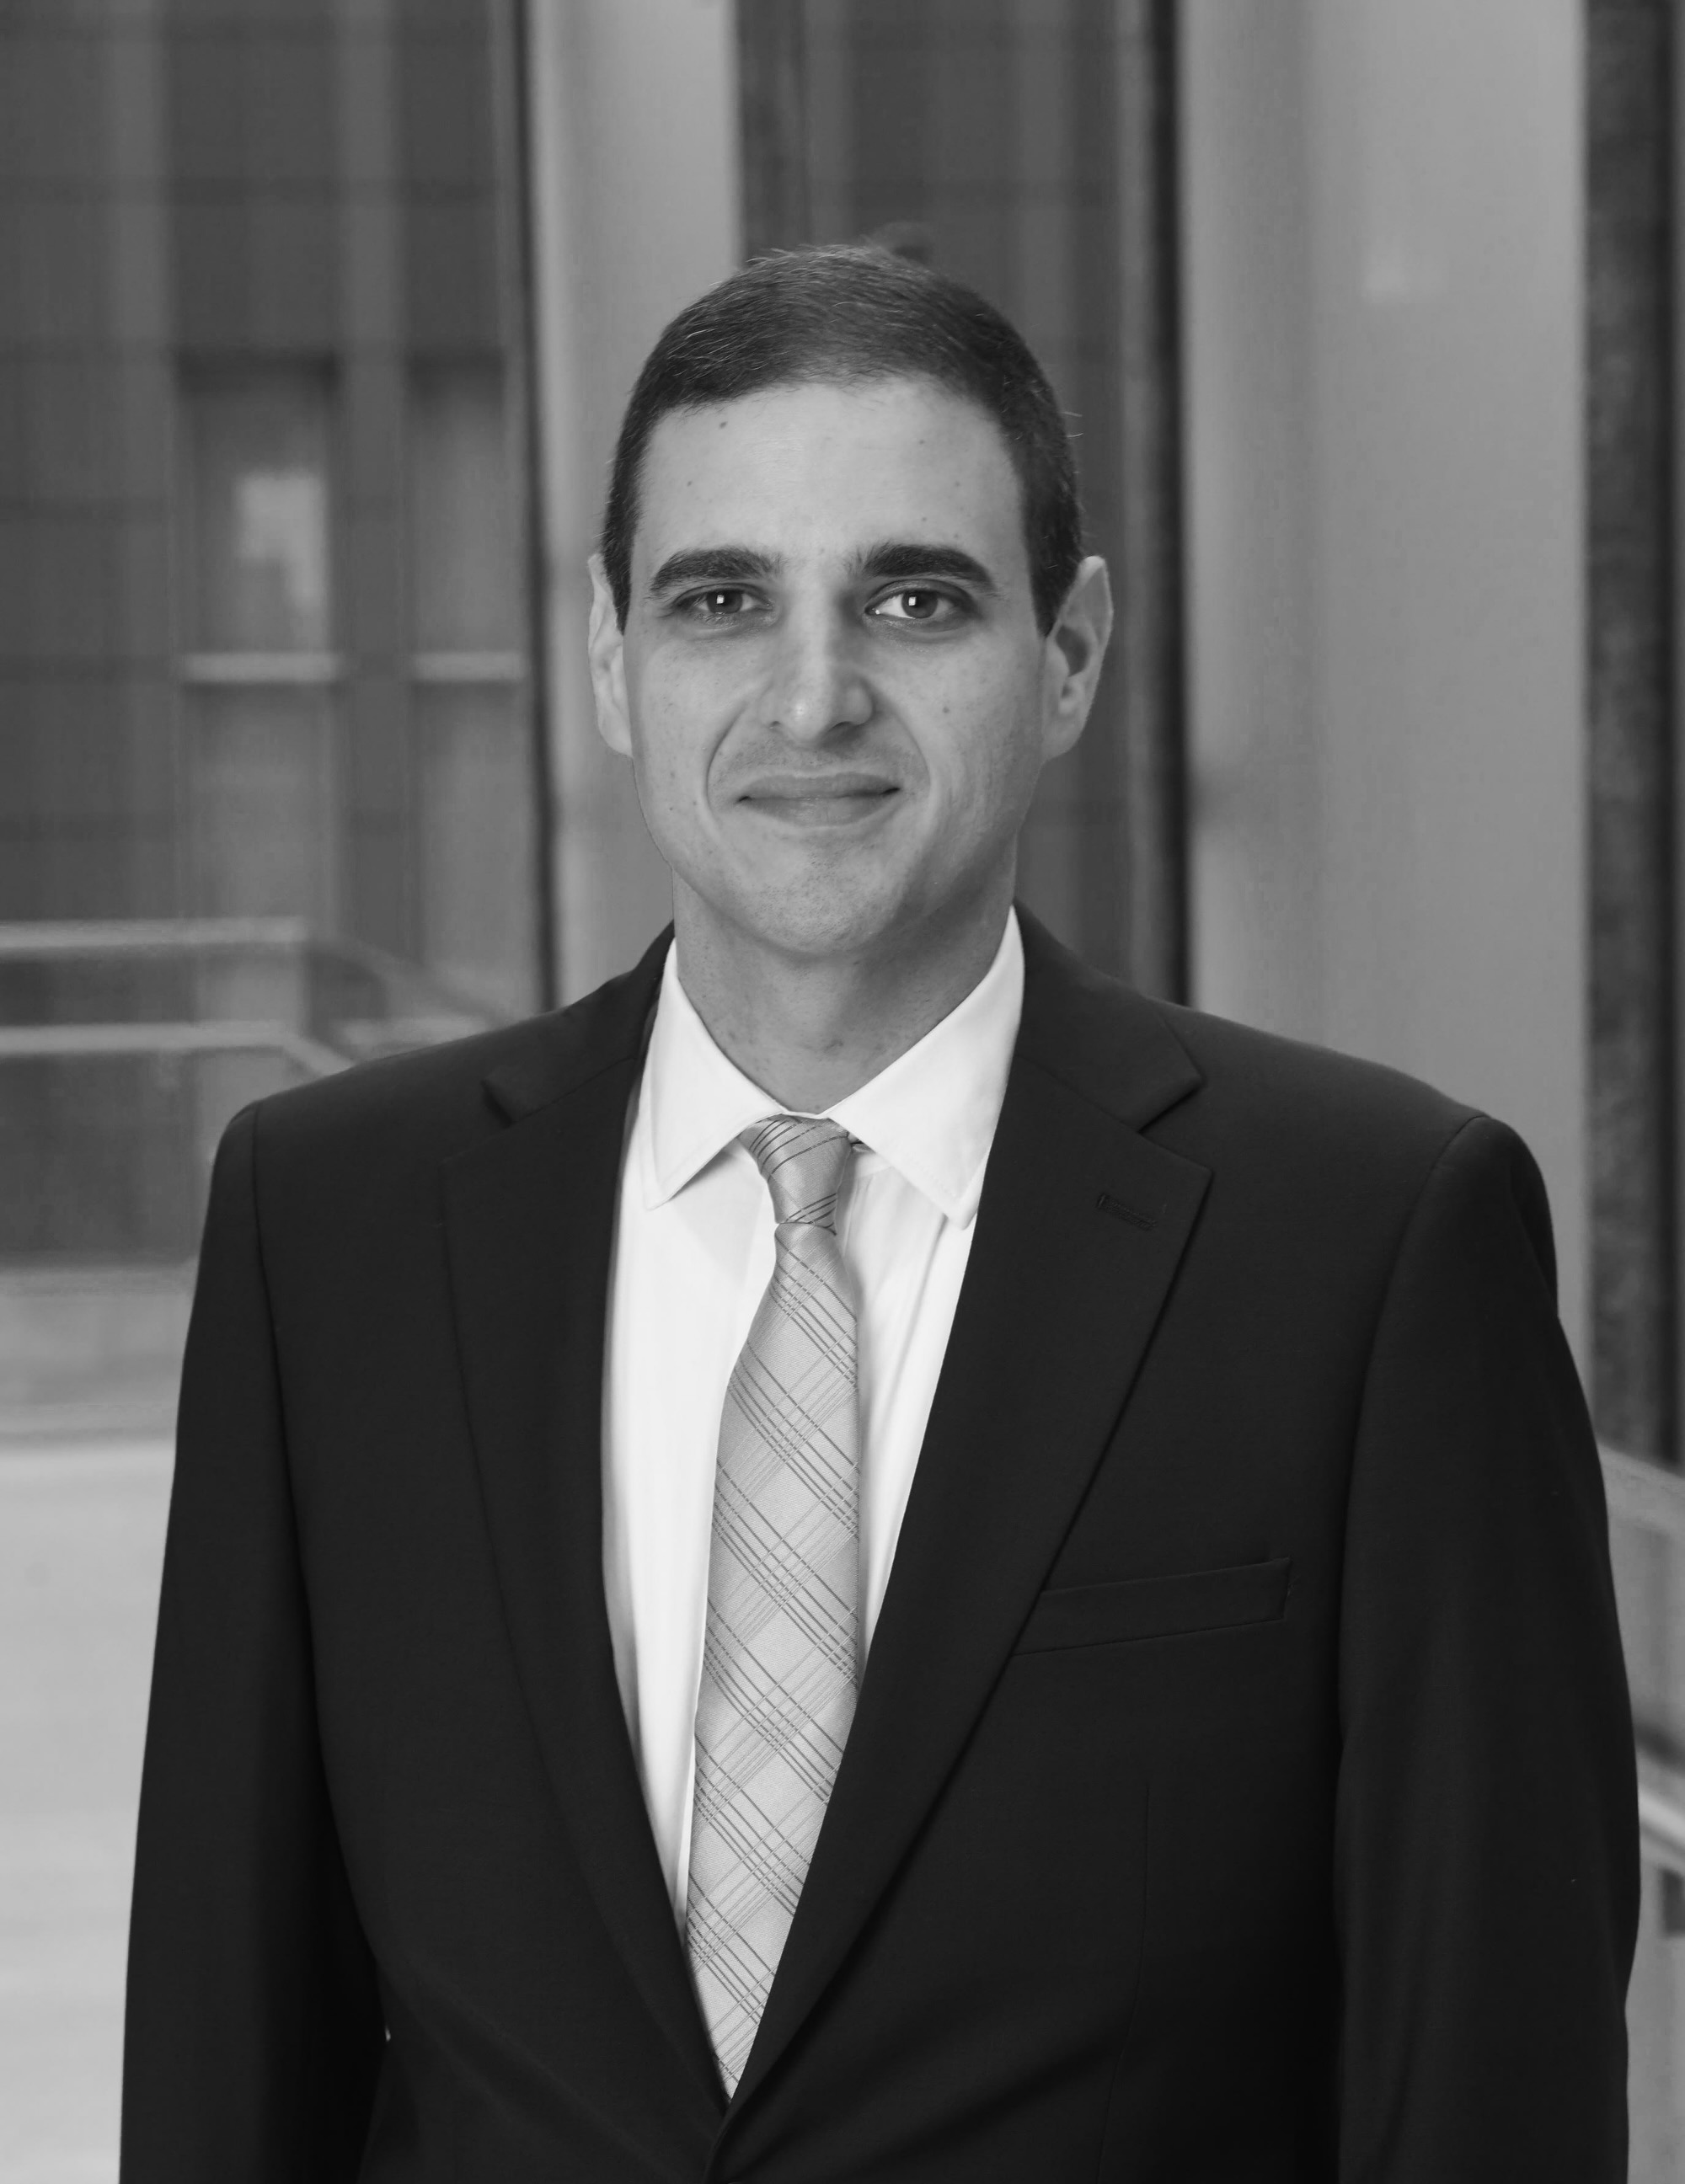
\includegraphics[width=0.4\linewidth]{fpic}

Hi! I'm Fuad

\hypertarget{current-policies-at-ross-and-umich}{%
\chapter{Current Policies at Ross and Umich}\label{current-policies-at-ross-and-umich}}

\hypertarget{university-policies}{%
\section{University Policies}\label{university-policies}}

\hypertarget{ross-policies}{%
\section{Ross Policies}\label{ross-policies}}

\hypertarget{publiclly-available-generative-ai}{%
\chapter{Publiclly Available Generative AI}\label{publiclly-available-generative-ai}}

\hypertarget{text}{%
\section{Text}\label{text}}

\hypertarget{images}{%
\section{Images}\label{images}}

\hypertarget{music}{%
\section{Music}\label{music}}

\hypertarget{video}{%
\section{Video}\label{video}}

\hypertarget{speech-synthesis}{%
\section{Speech Synthesis}\label{speech-synthesis}}

\hypertarget{organizational-challanges}{%
\chapter{Organizational Challanges}\label{organizational-challanges}}

\hypertarget{current-responses}{%
\section{Current Responses}\label{current-responses}}

\hypertarget{future-plans}{%
\section{Future Plans}\label{future-plans}}

\hypertarget{individual-challanges}{%
\chapter{Individual Challanges}\label{individual-challanges}}

\hypertarget{current-responses-1}{%
\section{Current Responses}\label{current-responses-1}}

\hypertarget{future-plans-1}{%
\section{Future Plans}\label{future-plans-1}}

\hypertarget{final-thoughts}{%
\chapter{Final Thoughts}\label{final-thoughts}}

\hypertarget{works-cited}{%
\chapter{Works Cited}\label{works-cited}}

\end{document}
